% ============================================================================
% October 9, 2026 build (agent draft). Replaces 05b_results.tex (Oct 6, base
% 15.07), whose numbers predate the 14.402 base and are not carried over.
% Sources, all at the 14.402 base, no new solves:
%   policy functions: output/model/jmp_slides_policy_functions_20261007/
%     child_policy.pdf, income_risk_policy.pdf (saved solution);
%   cost of a first child: latex/JMP_slides/frames/cost_of_a_first_child.pdf;
%   income risk at 2007: rental_menu_precaution_20261007/tables_price_tests.md;
%   2023 fixed-price battery: output/model/fixed_price_2023_battery_20261009/
%     (RESULTS.md, tables_2023_credit.md, bars_2023/loan_vs_insurance_bars.pdf);
%   mortgage credit and starter homes: deck frame
%     frame_mortgage_credit_starter_homes.tex and its sources;
%   PSID starter-home empirics: notes/starter_home_trap_empirics_20261009.md;
%   ranking of claims: notes/housing_tenure_claims_20261009.md.
% ============================================================================
\providecommand{\mocktodo}[1]{\textcolor{red}{[TODO: #1]}}

\section{Space, Credit and the Timing of Births}
\label{sec:results}

This section uses the calibrated model to ask which features of housing
shape fertility. I first describe how a household's choices change when a
first child arrives, and why the cost of the space a child requires bears
most heavily on households without savings. I then change, one at a time,
the price of space, access to credit, and household resources in the 2023
economy, holding prices fixed, and compare their effects on births. The
results organize around one distinction. Changes in the per-period cost of
the space a child requires, or in the buffer a household holds against that
cost, change how many children are born. Changes in the one-time cost of
getting into space, such as the down payment, change when households buy and
when they have children, and leave completed fertility within about one
percent.

\subsection{Household choices at the first birth}
\label{sec:results-policy-functions}

Figure~\ref{fig:results-policy} shows the choices of a childless renter aged
26 to 29 with middle earnings, as a function of its liquid wealth, in the
period in which it has no child and in the period in which a first child has
just been born. Without savings, the child pushes the household to the
largest rental unit, six rooms, and delays buying. With savings, the household
buys a larger home when the child arrives. Consumption falls when the child
arrives at every level of wealth. The value of trying for a child is negative
near the borrowing limit and turns positive with a small buffer, which is why
the probability of trying rises steeply with wealth at low wealth and is flat
above it.

\begin{figure}[t]
\centering
\includegraphics[width=0.85\linewidth]{../../output/model/jmp_slides_policy_functions_20261007/child_policy.pdf}
\caption{Choices with and without a first child}
\label{fig:results-policy}
\par\smallskip
\begin{minipage}{0.92\linewidth}
\footnotesize\textit{Notes:} Childless renter, age 26--29, middle earnings
state, 2007 steady state. Rooms, consumption, the probability of trying for a
child and the value of trying, by liquid wealth, in the period with no child
and with a first child just born.
\end{minipage}
\end{figure}

Figure~\ref{fig:results-cost} measures the housing cost of a first child for
childless renters of the same age without savings, at each level of earnings.
A first child raises the space the household occupies by up to two rooms.
Because renters cannot borrow, the extra rent is paid out of current income,
and at the lowest earnings consumption falls by 31 percent. The housing cost
of a child is therefore not a cost paid once but a commitment to a flow of
rent for as long as the child is at home, and it is largest relative to
income for the households that are least able to smooth it.
% [MODEL] budget_table_b0_age26_29.json (build_mechanism_readouts.py).

\begin{figure}[t]
\centering
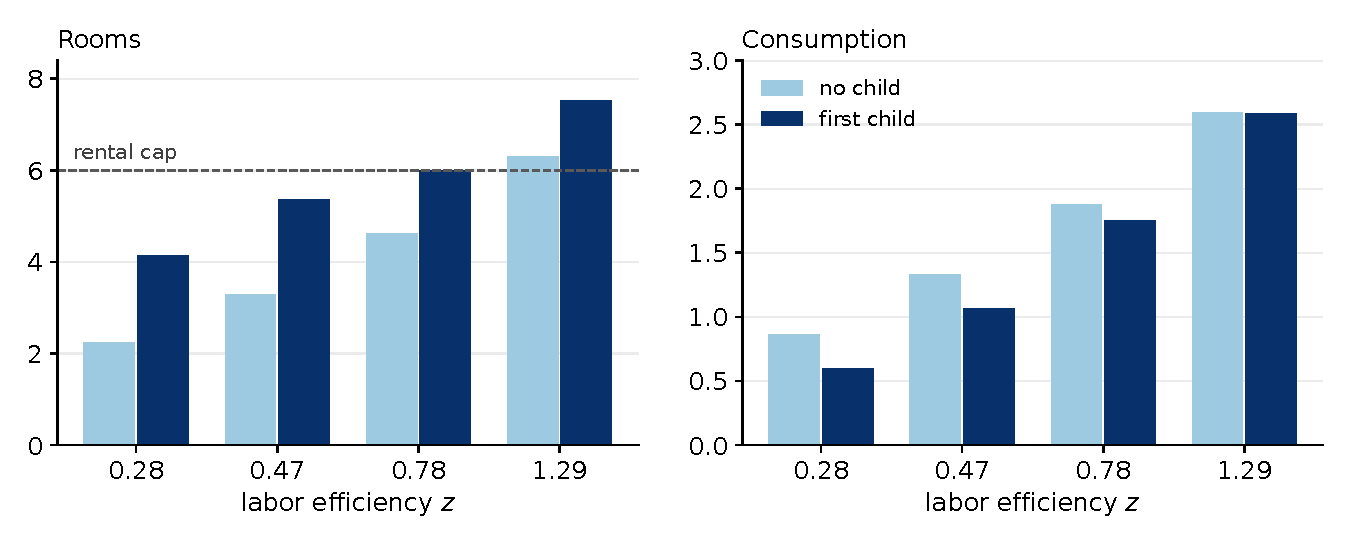
\includegraphics[width=0.85\linewidth]{../JMP_slides/frames/cost_of_a_first_child.pdf}
\caption{The housing cost of a first child}
\label{fig:results-cost}
\par\smallskip
\begin{minipage}{0.92\linewidth}
\footnotesize\textit{Notes:} Childless renters, age 26--29, no savings, by
labor efficiency $z$: rooms and consumption this period without and with a
first child. Rooms and consumption are averages over the tenure choice.
\end{minipage}
\end{figure}

A commitment to a flow of rent makes earnings risk a deterrent to
parenthood. Figure~\ref{fig:results-risk} lowers the standard deviation of
earnings innovations from 0.48 to 0.35 and plots the probability of a first
birth of a childless renter aged 26 to 29 with middle earnings. Without
savings, the probability rises from 0.41 to 0.58. With a buffer the two
curves meet: risk deters births mainly among households without savings.
Across all households, at the 2007 prices, completed fertility rises by 19
percent and childlessness falls from 19.0 to 7.4 percent. The effect of risk
grows with the commitment: in matched states, halving the variance of
earnings innovations raises first-birth attempts at ages 22 to 33 by 27.5,
38.7 and 51.1 percent with the space requirement at 80, 100 and 120 percent
of its calibrated value.
% [MODEL] completed 1.866 -> 2.220, childless 0.190 -> 0.074 (cells A6 vs
% A6_riskA); round4_tables_commitment_hazard_decomposition.md; the attempt
% numbers are confirmed in notes/housing_tenure_claims_20261009.md (claim 4).
\mocktodo{the risk experiment is large and its levels are not certified on a
clean risk solve; report a range, and rerun the floor-versus-one-time-cost
comparison at the production point to separate a commitment from a cost. The
baseline cell has completed fertility 1.866, not the calibrated 2.10, so
these cells are fixed-price cells, not the production steady state.}

\begin{figure}[t]
\centering
\includegraphics[width=0.6\linewidth]{../../output/model/jmp_slides_policy_functions_20261007/income_risk_policy.pdf}
\caption{Income risk and the probability of a first birth}
\label{fig:results-risk}
\par\smallskip
\begin{minipage}{0.92\linewidth}
\footnotesize\textit{Notes:} First-birth probability of a childless renter,
age 26--29, middle earnings, by liquid wealth, with the standard deviation of
four-year earnings innovations at its calibrated value, 0.48, and at 0.35.
Prices fixed at the 2007 steady state.
\end{minipage}
\end{figure}

\subsection{Credit, transfers and the price of space in 2023}
\label{sec:results-2023}

I now start from the 2023 economy of Section~\ref{sec:quant-2023} and make
one permanent, unanticipated change at a time. House prices, rents, the
pension and the rebate stay on their baseline paths, so each experiment
isolates the household response; any outlay is unfunded. I measure births in
2023 and completed fertility of the households aged 18 to 21 in 2023, their
mean number of children ever born at ages 46 to 49. Figure~\ref{fig:results-bars}
and Table~\ref{tab:results-2023} report the results.

\begin{figure}[t]
\centering
\includegraphics[width=\linewidth]{../../output/model/fixed_price_2023_battery_20261009/bars_2023/loan_vs_insurance_bars.pdf}
\caption{Credit, transfers and the price of space in 2023}
\label{fig:results-bars}
\par\smallskip
\begin{minipage}{0.92\linewidth}
\footnotesize\textit{Notes:} Change in completed fertility of the cohort
aged 18--21 in 2023 (left) and in its ownership at ages 18--29 (right),
relative to the baseline path. House prices and rents held on the baseline
path; one policy per row.
\end{minipage}
\end{figure}

\begin{table}[t]
\centering
\caption{Responses to housing costs, credit and transfers, 2023}
\label{tab:results-2023}
\small
\begin{tabular}{lrrr}
\toprule
 & Births, 2023 (\%) & Completed fertility (\%) & Ownership 18--29 (pp) \\
\midrule
House prices and rents $-10\%$ & $+4.7$ & $+7.0$ & $+2.5$ \\
Financed share $80\%\to95\%$ & $+0.8$ & $-1.0$ & $+25.7$ \\
Renter credit, 1 year of earnings & $+4.0$ & $+0.5$ & $-10.2$ \\
Renter credit, 2 years of earnings & $+5.8$ & $-0.8$ & $-13.5$ \\
Same total cost, paid to everyone & $+8.1$ & $+8.2$ & $+0.4$ \\
Lower income risk & $+24.2$ & $+23.6$ & $-0.1$ \\
\bottomrule
\end{tabular}
\par\smallskip
\begin{minipage}{0.92\linewidth}
\footnotesize\textit{Notes:} Changes relative to the baseline two-shock path
from 2023. Completed fertility: mean children ever born at 46--49 of
households aged 18--21 in 2023, three or more top-coded at three. Renter
credit allows renters to borrow up to one or two years of median earnings at
age 22. The transfer pays every household 0.097 per period, 3.3 percent of
mean income, the same total cost as the two-year renter credit. Lower income
risk: as in Figure~\ref{fig:results-risk}.
\mocktodo{the transfer paid only when earnings are low is pending; at 2007 it
raises completed fertility by 14.7 percent.}
\end{minipage}
\end{table}

Lower prices of space raise fertility substantially. With house prices and
rents 10 percent lower, completed fertility rises by 7.0 percent, about as
much as an unfunded transfer to every household worth 3.3 percent of mean
income (8.2 percent). Ownership of the young barely moves. The two
experiments act on the same margin: a lower rent of a room lowers the flow
cost of the space requirement, and a transfer raises the resources out of
which it is paid. The response to cash, about 2.5 percent more completed
fertility per percent of income, is of the same order as the
quasi-experimental estimates of the effect of child benefits.

Credit moves the timing of births, not their number. Raising the financed
share from 80 to 95 percent raises ownership of the young by 26 percentage
points, raises births in 2023 by 0.8 percent, and lowers completed fertility
by 1.0 percent. Credit to renters, which lets them borrow against future
earnings, raises births on impact by 4 to 6 percent and leaves completed
fertility within one percent of the baseline, consistent with households that
were waiting for a buffer having their children sooner. Both forms of credit change the
one-time cost of getting into space, the equity a buyer must hold or the
wealth a renter needs before a child, and neither changes the per-period
rent of a room, which equals the owner's user cost and does not depend on
the loan-to-value ratio. In the model, a mortgage lets a household own its
rooms sooner; it does not make those rooms cheaper to occupy.

The same distinction appears within the house price. Raising the price by
10 percent at an unchanged rent, starting from 2007, raises births on impact
by 1.1 percent and leaves completed fertility unchanged ($-0.02$ percent),
while raising both the price and the rent lowers births by 4.4 percent and
completed fertility by 5.3 percent. The response to the price at a given rent
comes from leveraged owners: births of owners whose equity is at most a
quarter of the value of their home rise by 5.0 percent, while those of
renters without savings fall by 0.1 percent. It is a change in timing.
% [MODEL] tables_capitalization.md (2007 state, rebate held); numbers
% confirmed in notes/housing_tenure_claims_20261009.md and
% notes/ptax_vs_credit_channels_20261009.md (section 2).

\subsection{Mortgage credit and starter homes}
\label{sec:results-starter}

Why does mortgage credit lower completed fertility at all, rather than leave
it unchanged? In the model, the households that credit brings into ownership
are young, childless and poor, and many of them buy the smallest home, two
rooms, which is below the space requirement and yields a parent essentially no
housing services. A household in such a home must move, and pay 6 percent of
the value to sell, before it can have a child. Table~\ref{tab:results-starter}
shows that this accounts for the effect. When the two- and four-room homes are
removed from the menu of homes for sale, the same increase in the financed
share raises ownership of the young by 4 points instead of 25, births in the
first period by 0.1 percent, and leaves completed fertility unchanged. With
the actual distribution of home sizes in the United States, credit leaves
completed fertility unchanged. Credit offered only to households that already
have children raises completed fertility by 1.2 percent; the gain is small
because parents can already rent a family-sized home.

\begin{table}[t]
\centering
\caption{Mortgage credit and the menu of homes for sale}
\label{tab:results-starter}
\small
\begin{tabular}{lrrr}
\toprule
Homes for sale & Ownership 18--29 & Births, first period & Completed fertility \\
\midrule
Without 2- and 4-room homes & 36\% $\to$ 40\% & $+0.1\%$ & $-0.05\%$ \\
With 2- and 4-room homes & 44\% $\to$ 69\% & $+0.4\%$ & $-1.4\%$ \\
\bottomrule
\end{tabular}
\par\smallskip
\begin{minipage}{0.92\linewidth}
\footnotesize\textit{Notes:} Financed share from 80 to 95 percent at fixed
house prices and rents, transfer held.
\end{minipage}
\end{table}

The starter-home mechanism is a feature of the model, not of the data. In the
model, 30 percent of young childless owners live in two rooms; in the PSID, 3
percent. And the PSID does not show the trap that the mechanism would
produce. Among couples with one child, those who own a home of at most four
rooms have the same probability of a second birth within two years as owners
of larger homes, a difference of $-0.9$ percentage points (standard error
3.5) on a base of 40 percent, and they are not stuck: 19 percent move to a
larger home within two years, against 11 percent of owners of large homes.
First-time buyers in the 2003--2007 boom bought homes of the same size as
earlier buyers, relative to their family, but paid 2.24 times their income
rather than 1.77: credit went into prices, not into smaller homes. The only
small-home gap in the data is at the first birth: childless first-time buyers
of small homes are 14 percentage points less likely to have a first child
within six years (standard error 6.7), which is as consistent with selection,
couples that do not plan children buying small, as with a trap. I therefore
read the effect of mortgage credit on completed fertility as zero to within
about one percent, and not as negative.
% [DATA] PSID-SHELF 1997-2019, code/data/starter_home_trap_20261009/.

The distinction between space and timing has one exception, and it confirms
the distinction. Credit raises fertility where it is the way into
family-sized space. If the largest rental unit had four rooms rather than
six, so that a family home had to be bought, lowering the required down
payment from 50 to 10 percent would raise completed fertility by 10.8
percent and lower childlessness from 24.9 to 18.5 percent; at the calibrated
six-room limit the same change lowers completed fertility by 1.0 percent while
raising young ownership from 22 to 62 percent. This is the direction of the
postwar mortgage expansion documented by
\citet{dettlingKearneyModernMortgage2025} and of the Brazilian housing lottery
of \citet{vandoornikFazioRamadoraiSkrastinsHousingFertility2025}, in which
credit raised family size. \citet{hacamoBabiesMortgageDeregulation2021} finds
that deregulation raised the joint probability of buying and having a child,
with no response among renters. The model reproduces the renter null and the
order of magnitude of the joint outcome; its birth response is of the same
order as his aggregate figure and far below his within-state estimate, and he
reports no completed-fertility estimate.
% [REVIEW Oct 10] notes/housing_tenure_claims_20261009.md ("stop saying" the
% model matches Hacamo) and notes/argument_for_corina_20261008.md, Oct 9
% correction; four-room numbers confirmed in RESULTS.md (cap 4, LTV 50 -> 90:
% completed +10.82%, childless 24.9 -> 18.5%; cap 6: -1.03%, own 18-29 21.8
% -> 62.0%).
\mocktodo{the four-room economy is not recalibrated (fixed prices, loss 942);
present this as a comparative static at a common price, and measure the size
distribution of rentals in the 1940 and 1950 Censuses of Housing before
mapping it to the postwar period.}
